% day3_seg1_navproblem/strapdown.tex
\begin{frame}
\frametitle{Inertial navigation Systems}
\framesubtitle{Strapdown Navigation:  Strapdown vs. Gimbaled}
\begin{itemize}
  \item Gimbaled INS:
  \begin{itemize}
	\item Gyro stabilized platform
	\item Gimbal assembly and torque motors
	\item Resolvers, slip rings, bearings, etc. to control  platform
	\item Goal: Maintain stable, locally level or inertial reference frame
  \end{itemize}
\end{itemize} 
\end{frame}


\begin{frame}
\frametitle{Strapdown Navigation: Strapdown vs. Gimbaled}
\begin{itemize}
  \item Gimbaled INS Issues
  \begin{itemize}
	\item Reliability and Cost: Lots of moving parts!
	\item Body rate and acceleration information not directly available
	\item Rate signals are generally noisy and have low bandwidth
  \end{itemize}
\end{itemize} 
\end{frame}


\begin{frame}
\frametitle{Strapdown Navigation: Strapdown vs. Gimbaled}
\begin{itemize}
  \item Strapdown INS:
  \begin{itemize}
	\item Inertial instruments strapped to body frame
	\item Requires local level accelerations to be computed using direction cosine matrix $\dcm{B}{L}$
	\item $\dcm{B}{L}$ derived from gyro-sensed body rates
    \item Strapdown systems can be implemented with either rate gyros or attitude gyros 
  \end{itemize} 
\end{itemize} 
\end{frame}

\begin{frame}
\frametitle{Strapdown Navigation: Strapdown vs. Gimbaled}
\begin{itemize}
  \item Strapdown INS Advantages
  \begin{itemize}
	\item Immediate detection of body rates and accelerations
	\item Fewer moving parts
	\item Potential redundancy advantages
  \end{itemize} 
  \item Gimbaled systems are nearly obsolete
\end{itemize} 
\end{frame}

\begin{frame}
\frametitle{Strapdown Inertial Block Diagram}
\begin{center}
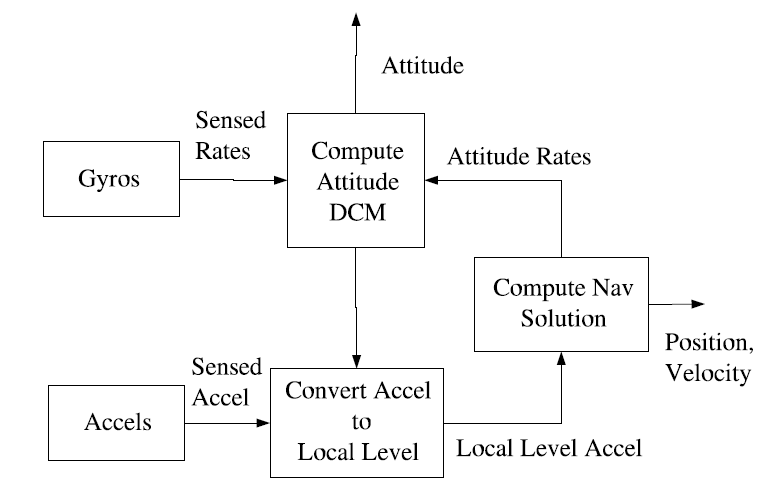
\includegraphics[scale=0.5]{graphics/strapdown_block.png}
\end{center}
\end{frame}

\begin{frame}
\frametitle{Basic Strapdown Navigation Equations}
 \begin{itemize}
 \item Need to compute attitude, velocity, and position
 \item I.e., need to compute $\dcm{B}{L}$ and $\dcm{L}{E}$
 \item These DCMs are dynamic quantities
 \item $\dcm{B}{L}$ determines attitude and can be rapidly varying
 \item $\dcm{L}{E}$ determines position and is slowly varying (relative to attitude dynamics)
\end{itemize}
\end{frame}


\begin{frame}
\frametitle{Strapdown Navigation Equations}
 \begin{itemize}
 \item Three differential equations
 \begin{itemize}
   \item Equation for body to local level transformation $\dcm{B}{L}$
   \item Equation for velocity (uses $\dcm{B}{L}$)
   \item Equation for local level to earth for position DCM $\dcm{L}{E}$
 \end{itemize}
\end{itemize}
\end{frame}

\begin{frame}
Strapdown Navigation Equations
 \begin{itemize}
 \item Two Algebraic Equations
 \begin{itemize}
   \item Equation for converting velocity to transport rate (to be explained)
   \item Equation for converting earth rate to local level
   coordinates
 \end{itemize}
\end{itemize}
\end{frame}
\begin{frame}
\frametitle{Strapdown Navigation Equations}
\framesubtitle{The Three Differential Equations}
\begin{equation}\label{cbleq}
  \cbleq
\end{equation}
\begin{equation}\label{strapveleq}
  \strapveleq
\end{equation}
\begin{equation}\label{cleeq}
  \cleeq
\end{equation}
\end{frame}

\begin{frame}
\frametitle{Strapdown Navigation Equations}
\framesubtitle{The Two Algebraic Equations}
\begin{equation}\label{trateeq}
  \trateeq \text{ (wander azimuth $\rho_z=0$)}
\end{equation}
\begin{equation}\label{erateeq}
  \erateeq
\end{equation}
\end{frame}

\begin{frame}
\frametitle{Strapdown Navigation Equations}
The $\dcm{B}{L}$ Equation \eqref{cbleq}
\[\cbleq\]
\begin{itemize}
\item All the $\Omega$ matrices represent rotation vector cross products in skew-symmetric matrix format
\begin{itemize}
 \item $\rotmat{I}{B}^B$ is rotational rate of aircraft in body
coordinates
\item $\rotmat{I}{E}^L$ is earth rate in local level coordinates
\item $\rotmat{E}{L}^L$ is transport rate in local level
coordinates
\end{itemize}
\end{itemize}
\end{frame}

\begin{frame}
\frametitle{Strapdown Navigation Equations: Detour into Cross Product Matrices}
\begin{itemize}
\item The cross product of $\omega=\colvecthree{\omega}{}$ with any other vector $v$ is the same as multiplying $v$ on the left by
$\Omega = \skewsymmat{\omega}{1}{2}{3}$
\item $\omega \times v=\Omega v$
\end{itemize}
\end{frame}

\begin{frame}
\frametitle{Strapdown Navigation Equations}
The $\dcm{B}{L}$ Equation \eqref{cbleq}
\[\cbleq\]
\begin{itemize}
\item Transport rate is the rotational rate of the aircraft due to
motion over the surface of the earth.  Is a function of velocity.
\item $\rotmat{I}{B}^B$ is total inertial angular rate sensed by gyros and includes effects of
transport and earth rates.
\item Hence transport and earth rate effects have to be subtracted
off.
\end{itemize}
\end{frame}

\begin{frame}
\frametitle{Strapdown Navigation Equations}
\framesubtitle{The Strapdown Velocity Equation} \eqref{strapveleq}
\[\strapveleq\]
 \begin{itemize}
 \item Sometimes referred to as the velocity rate equation
 \item $\specforce^B$ is specific force sensed by accelerometers in
 body coordinates (because the accels are strapped to the body --
 hence the term strapdown)
\end{itemize}
\end{frame}

%\begin{frame}
%\includegraphics[width=10in,height=6.5in]{strapnav_block.png}
%\end{frame}

\begin{frame}
\frametitle{Strapdown Navigation Equations}
\framesubtitle{The Transport Rate Equation}
 \eqref{cleeq}
\[\cleeq\]
\begin{itemize}
  \item Connected to velocity rate equation by the first algebraic equation \eqref{trateeq}:
\[\trateeq\]
  \item Eq. \eqref{cleeq} Sometimes referred to as position rate equation, because $\dcm{L}{E}$ directly implies the vehicle position
\end{itemize} 
\end{frame}

\begin{frame}
\frametitle{Strapdown Navigation Equations}
\framesubtitle{Position Rate / Transport Rate Equations (Geographic)}
\begin{itemize}
  \item North transport rate:
\begin{equation}\label{trateneq}
\trateneq
\end{equation} 
  \item East transport rate:
\begin{equation}\label{trateeeq}
\trateeeq
\end{equation} 
where $e$ is ellipticity (approx. $\dfrac{1}{298}$) and $R_e$ is mean equatorial earth radius
\end{itemize} 
\end{frame}

\begin{frame}
\frametitle{Strapdown Navigation Equations}
\framesubtitle{Position Rate / Transport Rate Equations (Geographic)}
\begin{itemize}
  \item Latitude Rate:
\begin{equation}\label{latrate}
\latrateeq
\end{equation}  
  \item Longitude Rate:
\begin{equation}\label{lonrate}
\lonrateeq
\end{equation}  
\end{itemize} 
\end{frame}

\begin{frame}
\frametitle{Strapdown Navigation Equations}
\begin{itemize}
  \item Geographic (north-slaved) mechanization has singularities at poles
  \item Two other approaches to local level coordinates:
  \begin{itemize}
	\item Free azimuth: vertical component of transport rate $\rho_z$= additive inverse of vertical component of earth rate
	\item Wander Azimuth:  vertical component of transport rate $\rho_z$ = 0
  \end{itemize}
\end{itemize} 
\end{frame}

\begin{frame}
\frametitle{Strapdown Navigation Equations}
\framesubtitle{Position Rate / Transport Rate Equations (Wander and Free Azimuth)}
\begin{itemize}
  \item X Transport Rate:
\begin{align}\label{xtrateeq}
\xtrateeq
\end{align}  
  \item Y Transport Rate:
\begin{align}\label{ytrateeq}
\ytrateeq
\end{align}  
\end{itemize} 
\end{frame}

\begin{frame}
\frametitle{Strapdown Navigation Equations}
\framesubtitle{Position Rate / Transport Rate Equations (Wander and Free Azimuth)}
\begin{itemize}
  \item Azimuth Rate:
\[
\rho_z= 
\begin{cases} 
-\erate d_{23}, &\text{if free azimuth;}\\ 
0,  &\text{if wander azimuth} 
\end{cases}
\]
  \item In equations above, the matrix $\left[d_{ij}\right]$ is the direction cosine matrix $\dcm{L}{E}$ from local level (L) frame to earth centered earth fixed (E) frame.
\end{itemize} 
\end{frame}
